% Options for packages loaded elsewhere
\PassOptionsToPackage{unicode}{hyperref}
\PassOptionsToPackage{hyphens}{url}
%
\documentclass[
]{book}
\usepackage{lmodern}
\usepackage{amssymb,amsmath}
\usepackage{ifxetex,ifluatex}
\ifnum 0\ifxetex 1\fi\ifluatex 1\fi=0 % if pdftex
  \usepackage[T1]{fontenc}
  \usepackage[utf8]{inputenc}
  \usepackage{textcomp} % provide euro and other symbols
\else % if luatex or xetex
  \usepackage{unicode-math}
  \defaultfontfeatures{Scale=MatchLowercase}
  \defaultfontfeatures[\rmfamily]{Ligatures=TeX,Scale=1}
\fi
% Use upquote if available, for straight quotes in verbatim environments
\IfFileExists{upquote.sty}{\usepackage{upquote}}{}
\IfFileExists{microtype.sty}{% use microtype if available
  \usepackage[]{microtype}
  \UseMicrotypeSet[protrusion]{basicmath} % disable protrusion for tt fonts
}{}
\makeatletter
\@ifundefined{KOMAClassName}{% if non-KOMA class
  \IfFileExists{parskip.sty}{%
    \usepackage{parskip}
  }{% else
    \setlength{\parindent}{0pt}
    \setlength{\parskip}{6pt plus 2pt minus 1pt}}
}{% if KOMA class
  \KOMAoptions{parskip=half}}
\makeatother
\usepackage{xcolor}
\IfFileExists{xurl.sty}{\usepackage{xurl}}{} % add URL line breaks if available
\IfFileExists{bookmark.sty}{\usepackage{bookmark}}{\usepackage{hyperref}}
\hypersetup{
  pdftitle={Conceitos e análises estatísticas com R e JASP},
  pdfauthor={Luis Anunciação (PUC-Rio), PhD},
  hidelinks,
  pdfcreator={LaTeX via pandoc}}
\urlstyle{same} % disable monospaced font for URLs
\usepackage{color}
\usepackage{fancyvrb}
\newcommand{\VerbBar}{|}
\newcommand{\VERB}{\Verb[commandchars=\\\{\}]}
\DefineVerbatimEnvironment{Highlighting}{Verbatim}{commandchars=\\\{\}}
% Add ',fontsize=\small' for more characters per line
\usepackage{framed}
\definecolor{shadecolor}{RGB}{248,248,248}
\newenvironment{Shaded}{\begin{snugshade}}{\end{snugshade}}
\newcommand{\AlertTok}[1]{\textcolor[rgb]{0.94,0.16,0.16}{#1}}
\newcommand{\AnnotationTok}[1]{\textcolor[rgb]{0.56,0.35,0.01}{\textbf{\textit{#1}}}}
\newcommand{\AttributeTok}[1]{\textcolor[rgb]{0.77,0.63,0.00}{#1}}
\newcommand{\BaseNTok}[1]{\textcolor[rgb]{0.00,0.00,0.81}{#1}}
\newcommand{\BuiltInTok}[1]{#1}
\newcommand{\CharTok}[1]{\textcolor[rgb]{0.31,0.60,0.02}{#1}}
\newcommand{\CommentTok}[1]{\textcolor[rgb]{0.56,0.35,0.01}{\textit{#1}}}
\newcommand{\CommentVarTok}[1]{\textcolor[rgb]{0.56,0.35,0.01}{\textbf{\textit{#1}}}}
\newcommand{\ConstantTok}[1]{\textcolor[rgb]{0.00,0.00,0.00}{#1}}
\newcommand{\ControlFlowTok}[1]{\textcolor[rgb]{0.13,0.29,0.53}{\textbf{#1}}}
\newcommand{\DataTypeTok}[1]{\textcolor[rgb]{0.13,0.29,0.53}{#1}}
\newcommand{\DecValTok}[1]{\textcolor[rgb]{0.00,0.00,0.81}{#1}}
\newcommand{\DocumentationTok}[1]{\textcolor[rgb]{0.56,0.35,0.01}{\textbf{\textit{#1}}}}
\newcommand{\ErrorTok}[1]{\textcolor[rgb]{0.64,0.00,0.00}{\textbf{#1}}}
\newcommand{\ExtensionTok}[1]{#1}
\newcommand{\FloatTok}[1]{\textcolor[rgb]{0.00,0.00,0.81}{#1}}
\newcommand{\FunctionTok}[1]{\textcolor[rgb]{0.00,0.00,0.00}{#1}}
\newcommand{\ImportTok}[1]{#1}
\newcommand{\InformationTok}[1]{\textcolor[rgb]{0.56,0.35,0.01}{\textbf{\textit{#1}}}}
\newcommand{\KeywordTok}[1]{\textcolor[rgb]{0.13,0.29,0.53}{\textbf{#1}}}
\newcommand{\NormalTok}[1]{#1}
\newcommand{\OperatorTok}[1]{\textcolor[rgb]{0.81,0.36,0.00}{\textbf{#1}}}
\newcommand{\OtherTok}[1]{\textcolor[rgb]{0.56,0.35,0.01}{#1}}
\newcommand{\PreprocessorTok}[1]{\textcolor[rgb]{0.56,0.35,0.01}{\textit{#1}}}
\newcommand{\RegionMarkerTok}[1]{#1}
\newcommand{\SpecialCharTok}[1]{\textcolor[rgb]{0.00,0.00,0.00}{#1}}
\newcommand{\SpecialStringTok}[1]{\textcolor[rgb]{0.31,0.60,0.02}{#1}}
\newcommand{\StringTok}[1]{\textcolor[rgb]{0.31,0.60,0.02}{#1}}
\newcommand{\VariableTok}[1]{\textcolor[rgb]{0.00,0.00,0.00}{#1}}
\newcommand{\VerbatimStringTok}[1]{\textcolor[rgb]{0.31,0.60,0.02}{#1}}
\newcommand{\WarningTok}[1]{\textcolor[rgb]{0.56,0.35,0.01}{\textbf{\textit{#1}}}}
\usepackage{longtable,booktabs}
% Correct order of tables after \paragraph or \subparagraph
\usepackage{etoolbox}
\makeatletter
\patchcmd\longtable{\par}{\if@noskipsec\mbox{}\fi\par}{}{}
\makeatother
% Allow footnotes in longtable head/foot
\IfFileExists{footnotehyper.sty}{\usepackage{footnotehyper}}{\usepackage{footnote}}
\makesavenoteenv{longtable}
\usepackage{graphicx,grffile}
\makeatletter
\def\maxwidth{\ifdim\Gin@nat@width>\linewidth\linewidth\else\Gin@nat@width\fi}
\def\maxheight{\ifdim\Gin@nat@height>\textheight\textheight\else\Gin@nat@height\fi}
\makeatother
% Scale images if necessary, so that they will not overflow the page
% margins by default, and it is still possible to overwrite the defaults
% using explicit options in \includegraphics[width, height, ...]{}
\setkeys{Gin}{width=\maxwidth,height=\maxheight,keepaspectratio}
% Set default figure placement to htbp
\makeatletter
\def\fps@figure{htbp}
\makeatother
\setlength{\emergencystretch}{3em} % prevent overfull lines
\providecommand{\tightlist}{%
  \setlength{\itemsep}{0pt}\setlength{\parskip}{0pt}}
\setcounter{secnumdepth}{5}
\usepackage{booktabs}
\usepackage{amsthm}
\makeatletter
\def\thm@space@setup{%
  \thm@preskip=8pt plus 2pt minus 4pt
  \thm@postskip=\thm@preskip
}
\makeatother
\usepackage[]{natbib}
\bibliographystyle{apalike}

\title{Conceitos e análises estatísticas com R e JASP}
\author{\href{mailto:\%20luisfca@puc-rio.br}{Luis Anunciação (PUC-Rio), PhD}}
\date{}

\begin{document}
\maketitle

{
\setcounter{tocdepth}{1}
\tableofcontents
}
\begin{Shaded}
\begin{Highlighting}[]
\NormalTok{knitr}\OperatorTok{::}\NormalTok{opts_chunk}\OperatorTok{$}\KeywordTok{set}\NormalTok{(}\DataTypeTok{echo =} \OtherTok{TRUE}\NormalTok{, }
                      \DataTypeTok{message =} \OtherTok{FALSE}\NormalTok{,}
                      \DataTypeTok{warning =} \OtherTok{FALSE}\NormalTok{,}
                      \DataTypeTok{fig.align=}\StringTok{"center"}\NormalTok{)}
\end{Highlighting}
\end{Shaded}

\hypertarget{prefuxe1cio}{%
\chapter{Prefácio}\label{prefuxe1cio}}

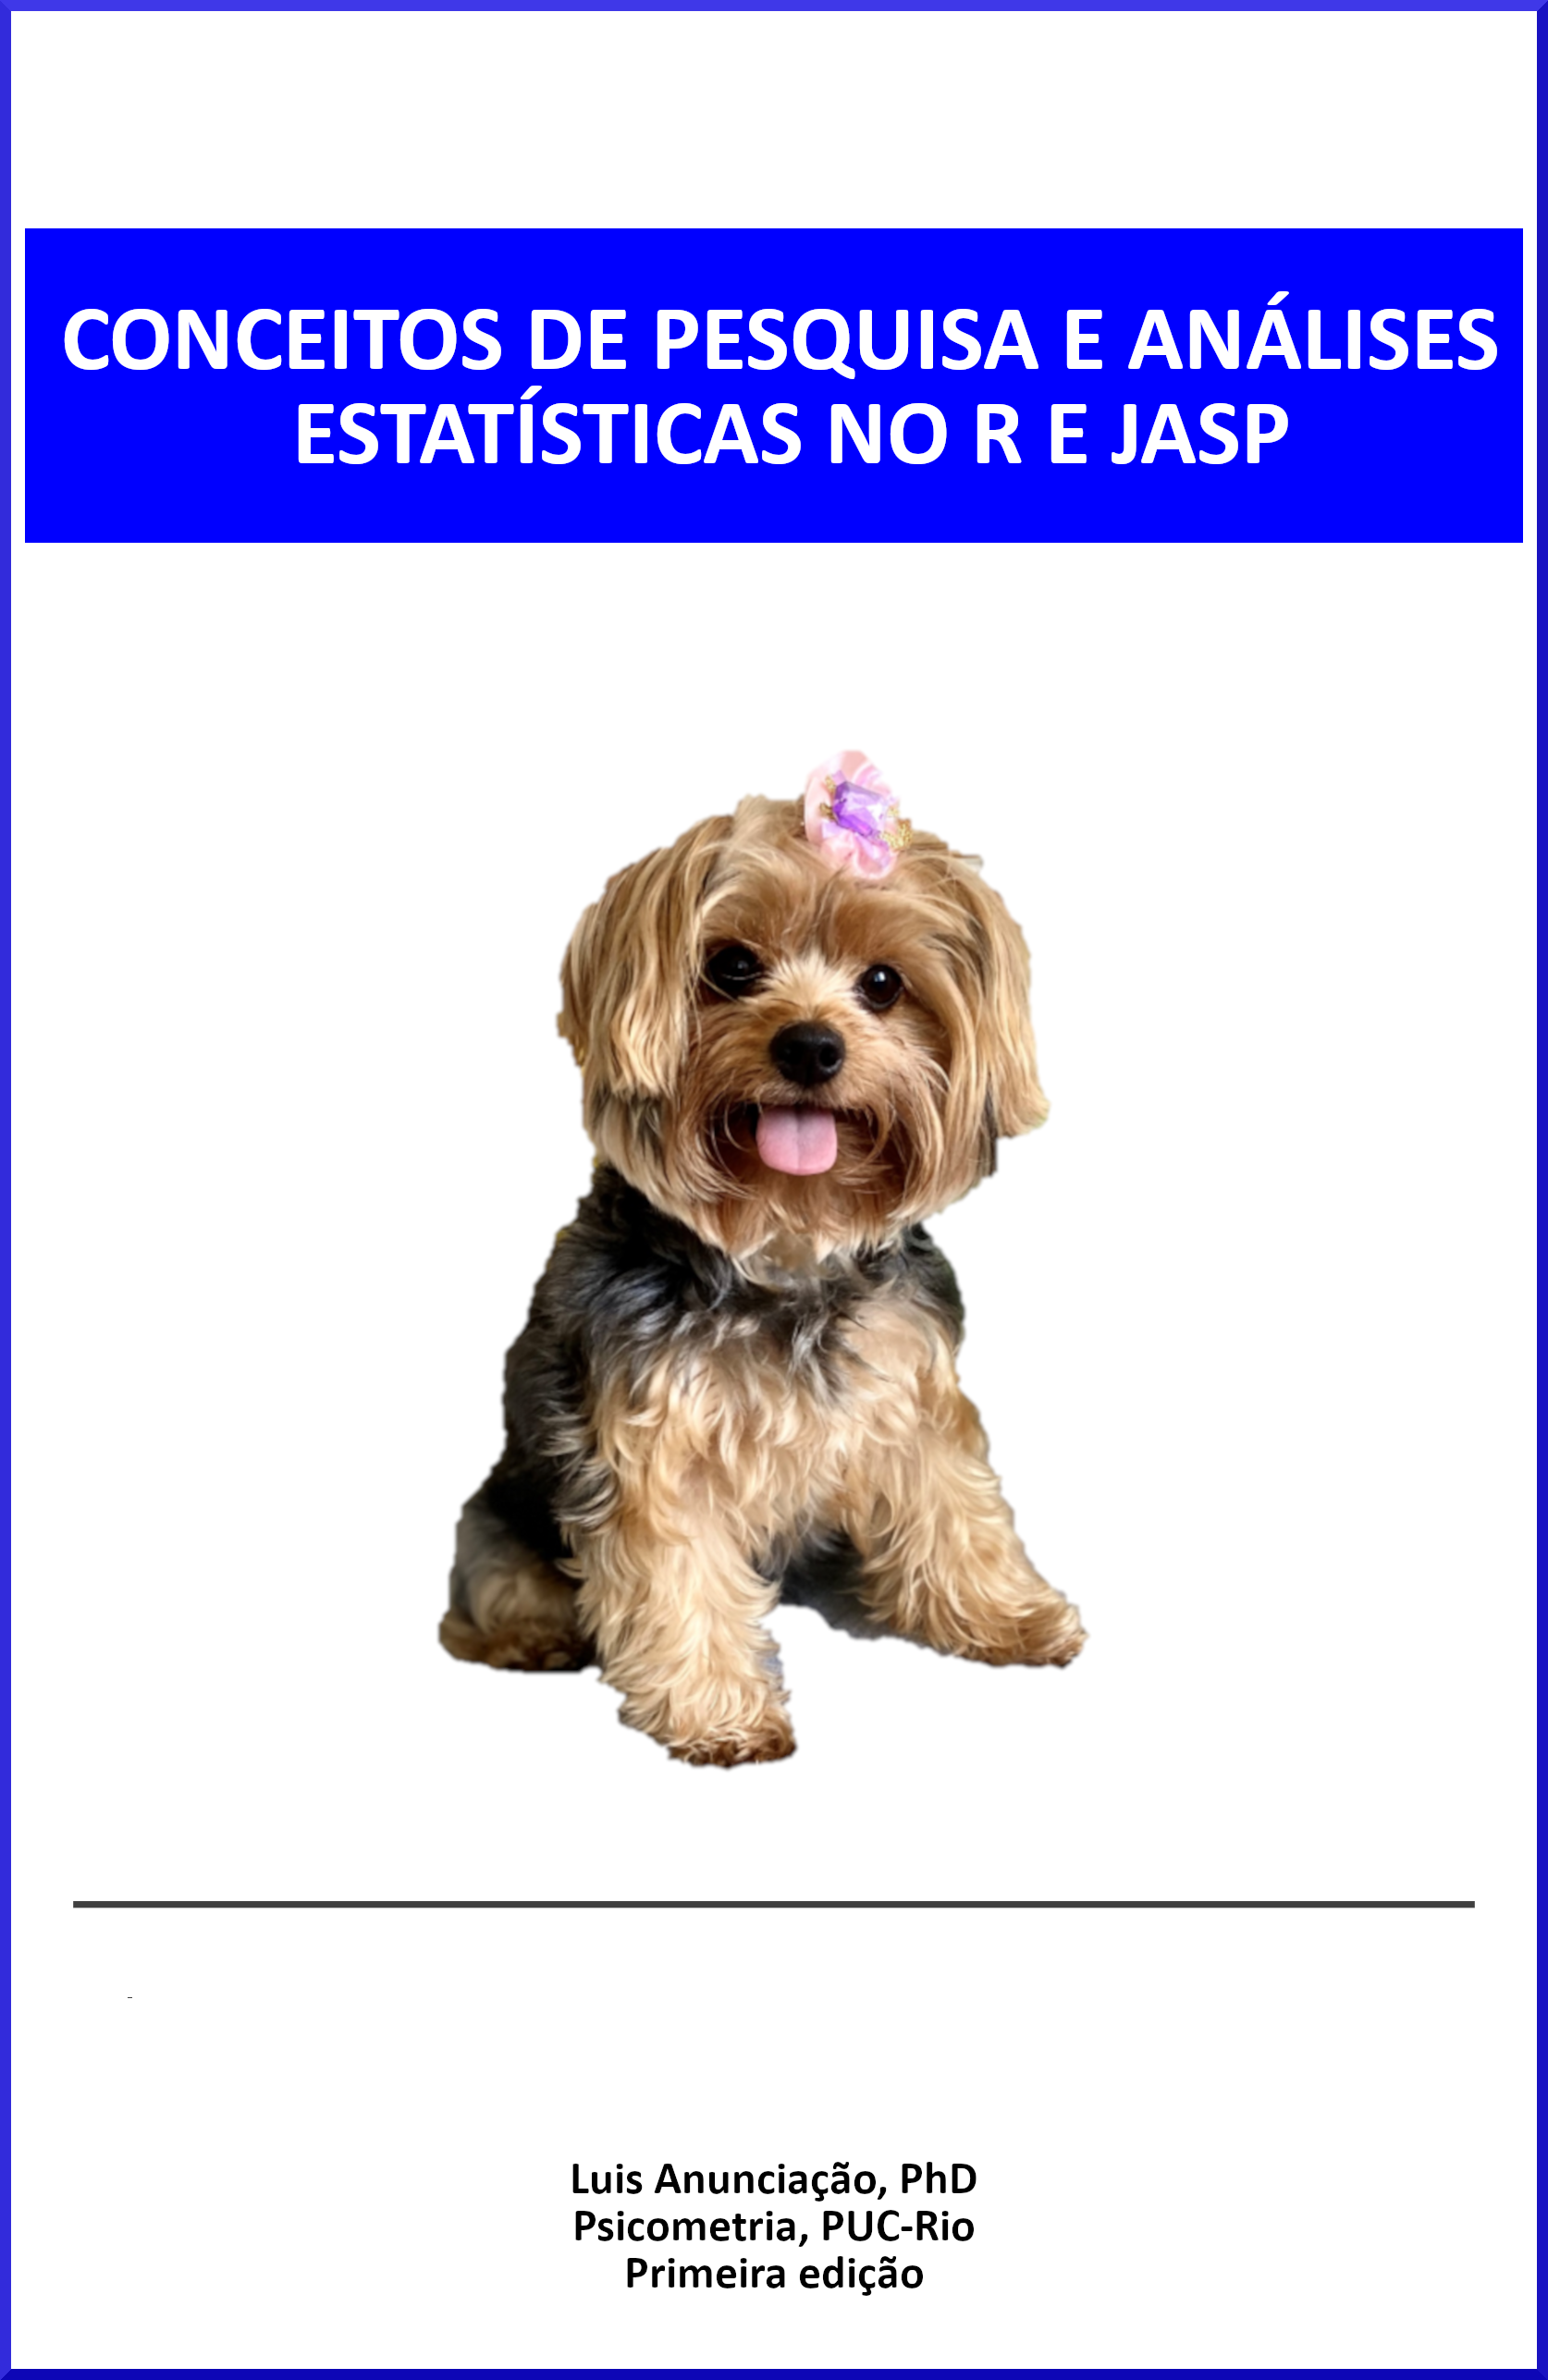
\includegraphics{./img/capa_jolie.png}
Atenção: Leia com cuidado. Este livro ainda está em sua fase de revisão.\\
Última modificação: 20 February, 2021

\hypertarget{a-proposta}{%
\section{A proposta}\label{a-proposta}}

Este livro nasceu como um dos principais e mais frutíferos frutos das aulas de graduação e pós-graduação ministradas por mim em alguns locais, mas com maior intensidade na PUC-Rio, UFRJ e IBNeuro. Por bastante tempo, nas aulas de estatística aplicada à Psicologia e Bioestatística, eu recorri a diferentes livros que, cada qual a sua maneira, apresentavam conceitos de pesquisa, técnicas estatísticas e análise de dados.

No entanto, acabei percebendo (ou tendo a impressão) de que eles apresentam a estatística por diferentes atalhos pedagógicos, (1) sugerindo que pesquisa e estatística eram áreas distantes, (2) que toda estatística podia ser resumida por testes de hipóteses independentes entre si e que (3) situações envolvendo dados reais não tinham tanto interesse. No geral, parece-me que para eles apresentarem a estatística na ciência, era necessário se distorcer pesadamente a ciência da estatística.

Em função disso, nos últimos anos, eu fui sentindo necessidade de apresentar os conceitos de pesquisa e técnicas estatísticas de forma integrada, contanto com dados reais e seguindo por uma metodologia de aula que pudesse ser pragmática, mas sem reforçar vícios inadequados sobre conceitos de estatística.

Conciliar essas condições em um único livro de maneira adequada é bastante improvável. Dessa forma, esse livro opta por uma abordagem majoritariamente pragmática, mas que evita se distanciar de conceitos teóricos. O pragmatismo é fundamental para que o estudante consiga, rapidamente, entender os procedimentos relacionados à análise de dados e implementar técnicas estatísticas para tomar decisões. Quão antes o estudante entender a utilidade da estatística para resolver problemas, maior é a probabilidade dele vir a gostar da área. Por sua vez, os aspectos teóricos são os alicerces para que o estudante possa perceber também que a utilidade que a estatística tem na ciência só é possível por ela ser uma disciplina sólida e robusta e que veio se aprimorando nas últimas décadas.

Isso posto, este livro é fruto de um grande esforço que tem a proposta de ser um manual técnico, em que são apresentados conceitos de pesquisa e análises estatísticas realizadas no R e no JASP e com especial aplicação em Psicologia e Bioestatística. Em cada capítulo, o estudante terá a oportunidade de acessar:

\begin{enumerate}
\def\labelenumi{\arabic{enumi}.}
\tightlist
\item
  Uma pesquisa científica, explicitando o problema e as hipóteses que a guiaram\\
\item
  O artigo publicado com os resultados\\
\item
  A base de dados em formato R ou CSV para reprodução das análises\\
\item
  O conjunto de procedimentos estatísticos utilizados\\
\item
  Recursos extras para aprofundamento em tópicos específicos\\
\item
  Exercícios que auxiliem no entendimento do conteúdo, quase sempre retirados de provas externas
\end{enumerate}

Com isso, o livro oferece ao estudante um ambiente em que ele possa resolver um problema real, utilizando as técnicas e métodos estatísticos como ferramentas para tomada de decisão. Apesar do foco ser mais no problema de pesquisa do que nas ferramentas analíticas, em todos os capítulos, a aplicação da estatística na ciência será reforçada pela apresentação de alguns conceitos da ciência da estatística.

Espero que este livro possa ser útil a estudantes de graduação e pós-graduação, agradável a leitores de estatística como de Psicologia e um recurso importante para outros docentes que, eventualmente, precisem de um material de apoio.

\hypertarget{objetivo}{%
\section{Objetivo}\label{objetivo}}

O livro tem como objetivos (1) apresentar, (2) discutir e (3) operacionalizar conceitos de pesquisa e análises estatística de dados a partir de pesquisas publicadas e dados reais. Espera-se que qualquer o estudante consiga realizar todas as ações descritas no decorrer dos capítulos de maneira guiada e intuitiva. As sintaxes utilizadas no ambiente R e as telas de execução do JASP são integralmente disponíveis.

\hypertarget{puxfablico-alvo}{%
\section{Público-alvo}\label{puxfablico-alvo}}

Este livro foi desenvolvido de maneira mais focada a estudantes de Psicologia e Bioestatística. As pesquisas e exemplos utilizados são mais aderentes a essas duas áreas. No entanto, como parte dos conceitos e análises implementadas no livro são interdisciplinares, espera-se que que estudantes de áreas como educação, administração e economia também possam também ter proveito do livro.

\hypertarget{formato-do-livro}{%
\section{Formato do livro}\label{formato-do-livro}}

O livro foi pensando para ter uma estrutura linear, formada por capítulos autossuficientes e desenvolvidos para responder questões específicas e pontuais. Acredito que, assim, ele possa atender tanto estudantes interessados em ler a obra inteira, como aqueles que buscam informações mais específicas sobre um tópico particular.

Esse formato adotado tende a gerar uma percepção diferente entre aqueles que consultarem apenas um capítulo ou outro e aqueles que lerem o conteúdo por completo. Há uma maior chance disso ocorrer em capítulos sobre testes estatísticos. Uma vez que diversos testes estatísticos são casos particulares de outros, alguns assuntos que parecer destoantes em uma leitura inicial, tornam-se articulados em outros capítulos.

Muitos capítulos recebem o nome de testes de hipóteses (ex: Teste T ou Regressão). Isso foi intencional e visa auxiliar estudantes que precisem apenas de informações pontuais, bem como tende a enfraquecer a ideia de uma relação ponto a ponto tipicamente feita entre testes estatísticos e delineamentos específicos.

\hypertarget{como-usar-este-livro}{%
\section{Como usar este livro}\label{como-usar-este-livro}}

O livro é formado por dois componentes: capítulos teóricos e capítulos voltados à análise de dados. Os capítulos teóricos reúnem alguns conceitos fundamentais de pesquisa e estatística, tais como tipos de variáveis, delineamento de pesquisa e técnicas de amostragem. Estes capítulos foram escritos pensando em alunos de graduação do curso de Psicologia. Tenho a impressão que esses capítulos serão pouco acessados, apesar de importantes.

Os capítulos analíticos são focados em testes de hipóteses e contam com uma metodologia direta ao ponto, em que atividades similares às realizadas nos artigos são demonstradas. Estes capítulos foram desenvolvidos para estudantes de pós-graduação. Acredito que esses capítulos serão bastante acessados.

A figura abaixo diagrama os dois componentes de forma aproximada.

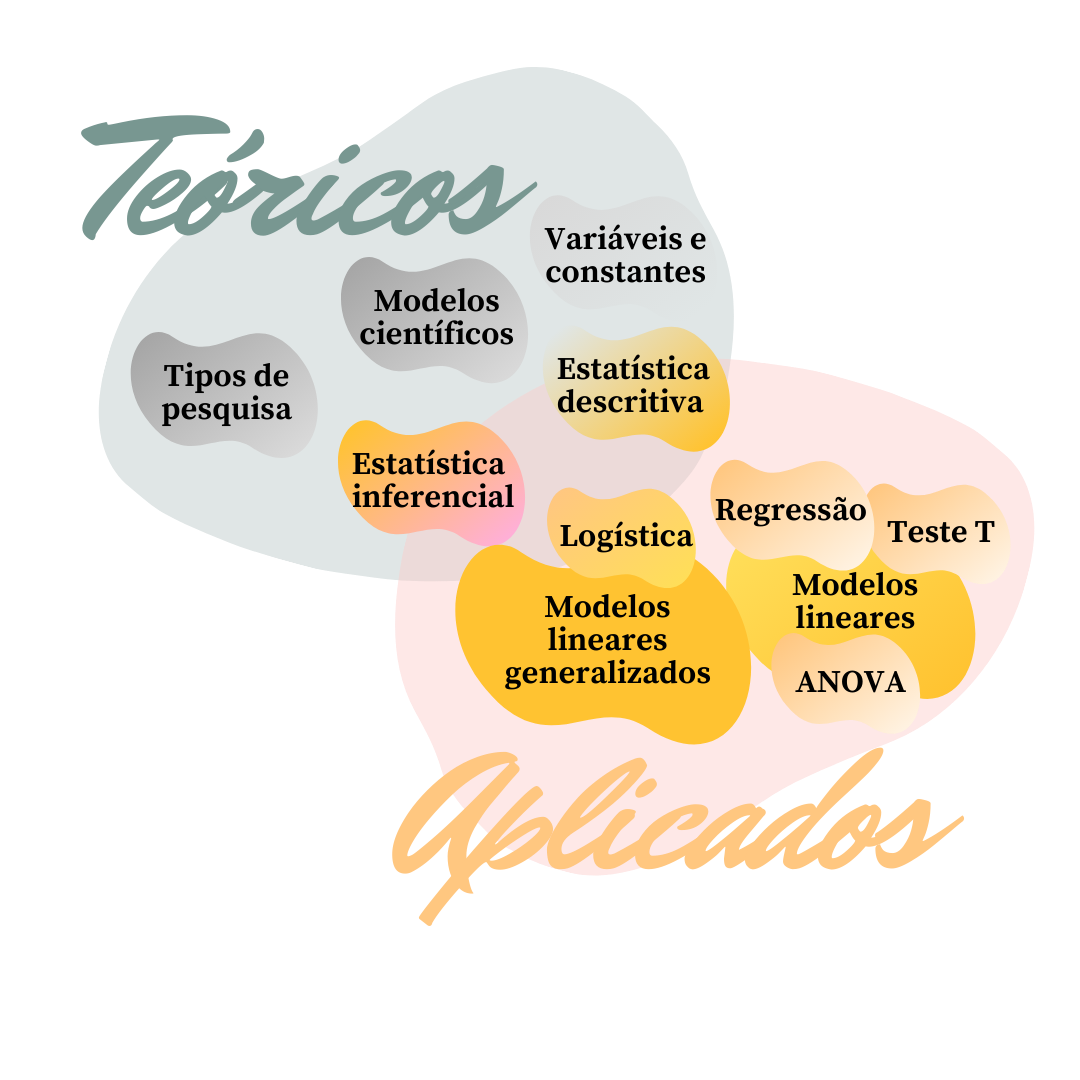
\includegraphics{./img/proposta.png}

\hypertarget{bases-de-dados}{%
\section{Bases de dados}\label{bases-de-dados}}

Todas as bases de dados utilizadas neste livro são \emph{Open Science}. Isso significa que elas são universalmente acessíveis, decorrentes de pesquisas empíricas e com artigos publicados. Eventualmente, alguns ajustes foram feitos às bases para torná-las mais acessíveis ou remover características de identificação.

Em cada capítulo, as bases irão aparecer na seção ``Pesquisa'', da seguinte maneira:

\begin{base}

A base desta pesquisa está disponível em formato \textbf{R (Rdata)} e em \textbf{CSV}, que é lido pelo JASP. Clique na opção desejada.

R Base: \href{}{Base R}\\
Base JASP : \href{}{Base CSV)}

\end{base}

As bases em R tem formato .RData e as bases para o JASP tem formato .CSV.

\hypertarget{o-r-e-os-pacotes}{%
\section{O R e os pacotes}\label{o-r-e-os-pacotes}}

O livro é integralmente desenvolvido pelo recurso de ``programação letrada'' no R Markdown, ou seja, ele entrelaça aspectos textuais e linhas de código. Em todos os capítulos, as funções nativas do R e do Tidyverse serão utilizadas. Caso alguém queira reproduzir as análises, será necessário apenas executar as linhas de código disponíveis no decorrer do livro.

O \texttt{tidyverse} costuma ter atualizações frequentes. Caso um alerta de \texttt{deprecated} seja apresentado, isso significa que a função utilizada foi parcialmente desativada, o que não costuma impactar nas análises.

\hypertarget{jasp}{%
\section{JASP}\label{jasp}}

O JASP é um programa gratuito que tem sido cada vez mais utilizado em Psicologia. Ele é feito integralmente por código aberto e sua interface é bastante amigável e intuitiva. Ao instalar o JASP, o R também será instalado em seu computador e ficará no pano de fundo. Dessa maneira, todas as ações feitas por \emph{Point and Click} no JASP, serão convertidas em linhas de código no R e apresentadas de maneira dinâmica no JASP.

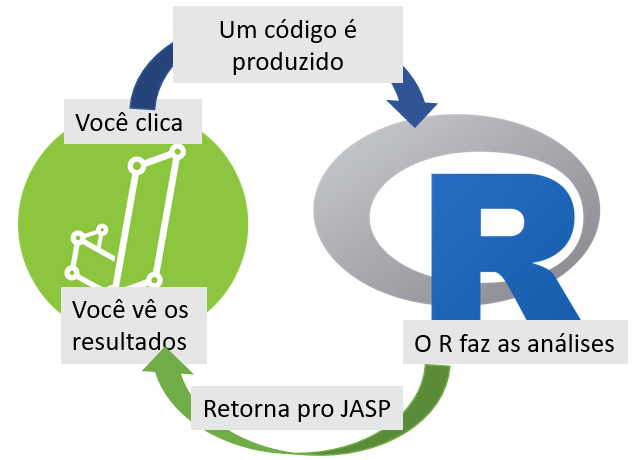
\includegraphics{./img/capa_r_jasp.png}

Em todos os capítulos, telas do JASP serão apresentadas para que seja possível a reprodução integral de algumas análises. Da mesma forma que qualquer pacotes estatístico, o JASP é atualizado frequentemente. Esse livro contou com a versão 0.14.1 e espero que futuras atualizações não comprometam a proposta do livro.

\hypertarget{outros-recursos}{%
\section{Outros recursos}\label{outros-recursos}}

Em cada um dos capítulos, aplicações da estatística e referências bibliográficas serão apresentadas. Tenha em mente que há um debate intenso em diferentes conceitos de estatística, da mesma forma que muitas condições computacionais podem aparecer durante a execução das análises propostas. Eu recomendo fortemente a comunidade \href{https://stackoverflow.com/}{stackoverflow} como um recurso pedagógico para auxiliar em ambos os cenários.

Quetões relacionadas aos capítulos são listadas de forma a conectar o conteúdo do livro com exigências balizadas por critérios externos, tal como o ENADE e bancas de concurso.

\hypertarget{capa}{%
\section{Capa}\label{capa}}

Por tradição, livros de Ciência de Dados e Estatística utilizam a imagem de algum animal na capa. Há livros com cachorros, papagaios, peixes, carangueijos, Lagartos, etc. Esse livro não foge dessa regra e tem como capa a Jolie, a minha cachorrinha com a Anna. Ela foi indispensável para o atraso ao término deste livro.

\hypertarget{versuxe3o-do-livro}{%
\section{Versão do livro}\label{versuxe3o-do-livro}}

Como todos os livros, este também tem uma história de desenvolvimento. A tabela abaixo apresenta a versão, a data de lançamento e algumas características importantes.

\begin{longtable}[]{@{}lll@{}}
\toprule
\begin{minipage}[b]{0.24\columnwidth}\raggedright
Versão\strut
\end{minipage} & \begin{minipage}[b]{0.34\columnwidth}\raggedright
Data\strut
\end{minipage} & \begin{minipage}[b]{0.34\columnwidth}\raggedright
Características\strut
\end{minipage}\tabularnewline
\midrule
\endhead
\begin{minipage}[t]{0.24\columnwidth}\raggedright
Beta 1\strut
\end{minipage} & \begin{minipage}[t]{0.34\columnwidth}\raggedright
Fevereiro, 2020\strut
\end{minipage} & \begin{minipage}[t]{0.34\columnwidth}\raggedright
Primeira versão. Baixa revisão textual e dos conceitos estatísticos. Erros são esperados. A utilização deve ser feita apenas de maneira incipiente\strut
\end{minipage}\tabularnewline
\bottomrule
\end{longtable}

\hypertarget{agradecimentos-e-revisuxf5es-tuxe9cnicas}{%
\section{Agradecimentos e revisões técnicas}\label{agradecimentos-e-revisuxf5es-tuxe9cnicas}}

Nenhum homem é uma ilha. Este livro só foi possível graças a um conjunto de pessoas que auxiliaram e fizeram uma profunda revisão do texto. Meus sinceros agradecimentos a (ao):

J. Landeira-Fernandez, PUC-Rio\\
Regina Albanense, CONRE\\
Cristiano Fernandes, PUC-Rio\\
Danilo Assis Pereira, IBNeuro\\
Ana Carolina de Almeida Portugal, UFRJ\\
Alunos da PUC-Rio, UFRJ, IBNeuro e ANOVA

\hypertarget{programas-estatuxedsticos}{%
\chapter{Programas estatísticos}\label{programas-estatuxedsticos}}

\begin{objectives}
\textbf{Objetivos do capítulo}\\
1. Apresentar os programas estatísticos utilizados durante o livro\\
2. Discutir características do R, tidyverse e seus pacotes\\
3. Discutir características do JASP
\end{objectives}

Programas estatísticos são ferramentas indispensáveis tanto na gestão, como na análise dos dados resultantes de uma pesquisa. Eles servem para otimizar o tempo gasto nas etapas analíticas de uma pesquisa, apesar de, em menor escala, permitirem a execução de análises inadequadas. No dia a dia de um pesquisador, apenas muito raramente as análises são feitas manualmente. Dessa maneira, o conhecimento de programas de análise de dados faz parte das competências esperadas para quem deseja ou precisa trabalhar com estatística.

Atualmente, há muitos programas e pacotes estatísticos disponíveis para uso. Acredito que a maioria deles tenham mais similaridades do que diferenças e produzam resultados confiáveis. Neste livro, o R e o JASP serão utilizados e algumas de suas características serão descritas neste capítulo.

\hypertarget{o-r}{%
\section{O R}\label{o-r}}

O R é uma linguagem de programação focada em análises estatísticas, que vem ganhando popularidade entre pesquisadores e cientistas. Este livro foi integralmente feito e baseado no ambiente R que, apesar de ainda não ser o programa mais frequente em Psicologia, apresenta diversas vantagens em comparação aos programas mais usuais.

\begin{itemize}
\item
  o R e todos os seus pacotes e otimizações são gratuitos.
\item
  o R é uma linguagem de programação desenvolvida especificamente para Estatística.

  \begin{itemize}
  \tightlist
  \item
    Diferente de uma linguagem mais geral (por exemplo, Python) ou de um programa \emph{point and click}, o R é uma linguagem focada em análise estatística. Ao se programar utilizando o R, o usuário tem controle total das ações realizadas e dos resultados obtidos. Assim, raramente o R apresentará resultados excessivos e distantes das análises solicitadas. Apesar disso poder assustar no início, acredito que essa característica seja essencial e, inclusive, serve como um excelente auxílio pedagógico para que o estudante planeje adequadamente as análises de interesse, em vez de apenas selecionar parte de um \emph{output} padronizado, como ocorre com o SPSS.
  \end{itemize}
\item
  O R é um programa de nicho em Estatística. Essa característica faz com que ele seja absolutamente adaptado para o dia a dia em estatística, incluindo não apenas análises descritivas e inferenciais, mas também análises para simulação e controle de resultados.
\item
  O R permite o desenvolvimento de interfaces web e aplicativos.
\item
  O R tem diversos pacotes.

  \begin{itemize}
  \tightlist
  \item
    Pacotes são complementos que permitem otimizar as análises que o R faz. A comunidade R tem um exército de pacotes, que além de gratuitos, foram verificados publicamente. O ambiente CRAN (\emph{The Comprehensive R Archive Network}) é o local em que estes pacotes estão alocados. Neste livro, todos os capítulos contam com pacotes específicos, que permitiram que análises complexas fossem realizadas com poucos comandos.
  \end{itemize}
\item
  O R possui uma enorme comunidade de apoio.

  \begin{itemize}
  \tightlist
  \item
    Os usuários do R formam uma rede muito dinâmica e que oferece grande apoio em caso das mais diversas dúvidas. A comunidade \href{https://stackoverflow.com/}{stackoverflow} talvez seja a mais voluma e reúne pessoas de todas as nacionalidades.
  \end{itemize}
\end{itemize}

Para baixar o R, é necessário ir no site \url{https://cran.r-project.org/}. Em seguida, para baixar o R Studio, é necessário acessar \url{https://rstudio.com/}.

\hypertarget{tidyverse}{%
\section{Tidyverse}\label{tidyverse}}

O Tidyverse é um ambiente de pacotes. Eles funcionam de maneira totalmente integrada e permitem que a estrutura da programação seja mais intuitiva e próxima à forma pela qual pensamos. No Tidyverse, os códigos seguem a lógica de sujeito + verbo e permitem uma programação encadeada, ao se utilizar a ligação \emph{pipe} (\texttt{\%\textgreater{}\%}). Ao instalar o tidyverse \texttt{install.package("tidyvese")}, os pacotes abaixo ficam disponíveis no R.

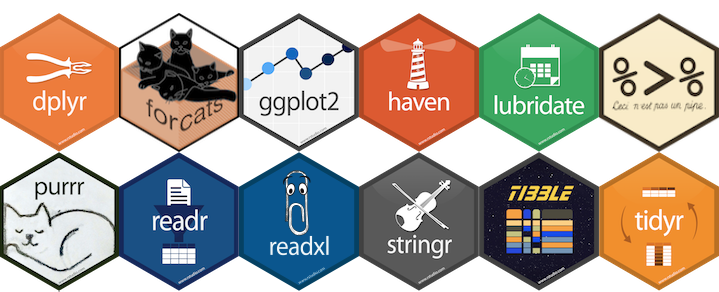
\includegraphics{./img/tidyverse_website.PNG}

\hypertarget{dificuldades-esperadas}{%
\section{Dificuldades esperadas}\label{dificuldades-esperadas}}

Algumas dificuldades são esperadas quando se trabalha programação no geral e com o R especificamente. Apesar do R e seus pacotes oferecem excelentes ferramentas para análise de dados, algumas condições descritivas são demasiadamente custosas. Por exemplo, enquanto realizar algumas tabelas e gráficos no Excel é tremendamente fácil, as vezes o R exige diversas linhas de código para isso.

Nesse sentido, na relação entre dificuldade e complexidade, o R sai na frente em tarefas complexas (como exemplo, estimar os coeficientes de um modelo não-linear), mas talvez perca em tarefas fáceis (por exemplo, gerar uma tabela de contingência). A Figura a seguir apresenta esta relação comparando as análises feitas no R e no Excel.

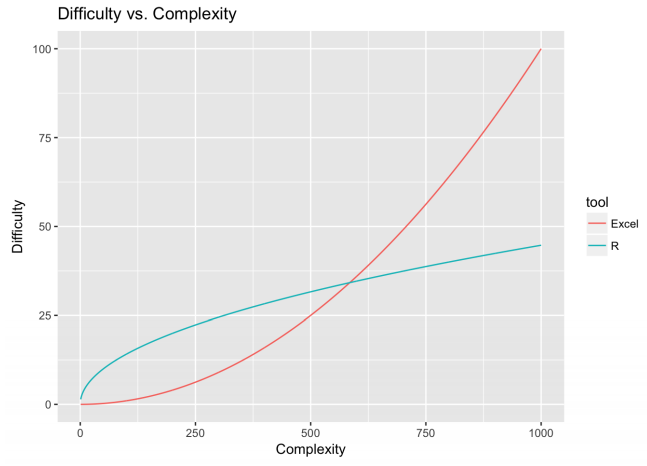
\includegraphics{./img/excel_r.PNG}

Além disso, o R traz uma outra barreira importante em aspectos que envolvam o ensino de estatística, especialmente na graduação. Como o R é uma linguagem de programação, o estudante teria de aprender a programar antes de conseguir entender conceitos de pesquisa e a utilidade da estatística. Isso poderia impactar negativamente na motivação do estudante, principalmente àqueles com uma aversão \emph{a priori} da matéria,

Em situações como esta, talvez o ideal seja começar motivando o estudante a entender como a estatística é uma ferramenta importante para tomar decisões para, só depois e lentamente, apresentar aspectos matemáticos e computacionais.

\hypertarget{verbos-do-dplyr}{%
\section{Verbos do dplyr}\label{verbos-do-dplyr}}

Entre os pacotes do ambiente tidyverse, o dplyr é o que será mais utilizado. Este pacote funciona de maneira muito intuitiva, em que as funções dependem de uma estrutura \texttt{sujeito\ \%\textgreater{}\%\ verbo(complemento)}. Essa é uma diferença importante em relação ao R Base. Por exemplo, no R Base é necessário executar \texttt{names(dataset)} para verificar as variáveis de um conjunto de dados. Pelo dplyr deve-se utilizar \texttt{dataset\ \%\textgreater{}\%\ names}.

O dplyr funciona a partir de verbos declarativos e os principais estão listados na tabela a seguir. As sintaxes deixadas no decorrer do livro também permitem uma melhor apreensão das funcionalidades.

\begin{longtable}[]{@{}ll@{}}
\toprule
Verbo & Ação\tabularnewline
\midrule
\endhead
glimpse & Inspeciona os dados\tabularnewline
count & Conta os níveis de uma variável\tabularnewline
select & seleciona uma variável específica\tabularnewline
filter & Filtra os resultados por um nível específico de uma variável\tabularnewline
group\_by & Agrupa os resultados por níveis de uma variávei específica\tabularnewline
summarise & Apresenta sumários (com medidas estatísticas)\tabularnewline
mutate & Cria novas variáveis ou altera as existentes\tabularnewline
arrange & Organiza a apresentação dos resultados\tabularnewline
left\_join & Junta bases ou colunas\tabularnewline
pivot\_longer & Transforma uma base larga em longa\tabularnewline
pivot\_wider & Transforma uma base longa em larga\tabularnewline
\bottomrule
\end{longtable}

\emph{Nota: Em alguns momentos, em função da praticidade computacional, algumas sintaxes vão contar com o formato base do R.}

É importante ficar atento às atualizações do dplyr e do sistema tidyverse como um todo. Eventualmente, mudanças podem ocorrer e impossibilitar (ou dificultar) a reprodução de rotinas antigas.

\hypertarget{o-jasp}{%
\section{O JASP}\label{o-jasp}}

O JASP é um programa gratuito, com uma interface amigável, \emph{point and click} e altamente versátil para a maioria das análises realizadas. A versão utilizada neste livro é a 0.14.1. O JASP foi desenvolvido por um time de psicólogos e estatísticos liderados pelo Prof.~Eric-Jan Wagenmakers, da Universidade de Amsterdam. Isso talvez explique o motivo pelo qual o JASP vem sendo cada vez mais utilizado em análises de dados psicológicos e na docência de matérias relacionadas a métodos estatísticos.

Para baixar o JASP, é necessário acessar \url{https://jasp-stats.org/download/}.

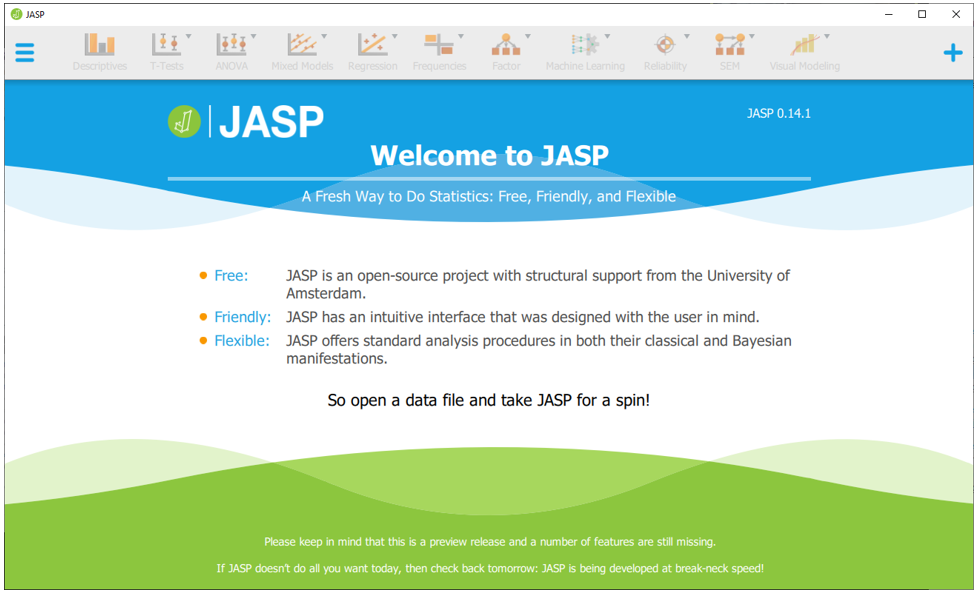
\includegraphics{./img/cap_jasp_interface.png}

Quando se instala o JASP no computador, se instala também o R. Todas as ações feitas no JASP se transformam em linhas de código que são enviadas ao R e, em seguida, retornam pro JASP e são apresentadas na tela. Isso ocorre de maneira instantânea e não há nenhum incômodo para o usuário. Na maioria das vezes, computadores pessoais conseguem rodar o JASP sem grandes problemas.

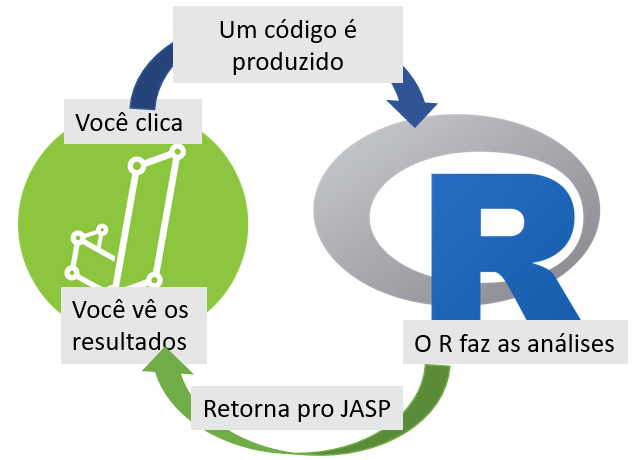
\includegraphics{./img/capa_r_jasp.png}

O idioma oficial do JASP é o inglês e, nesta versão, não pode ser alterado. Para fazer qualquer análise, é necessário carregar um arquivo de dados. Isso pode ser feito no símbolo das três linhas, localizado na parte superior à esquerda.

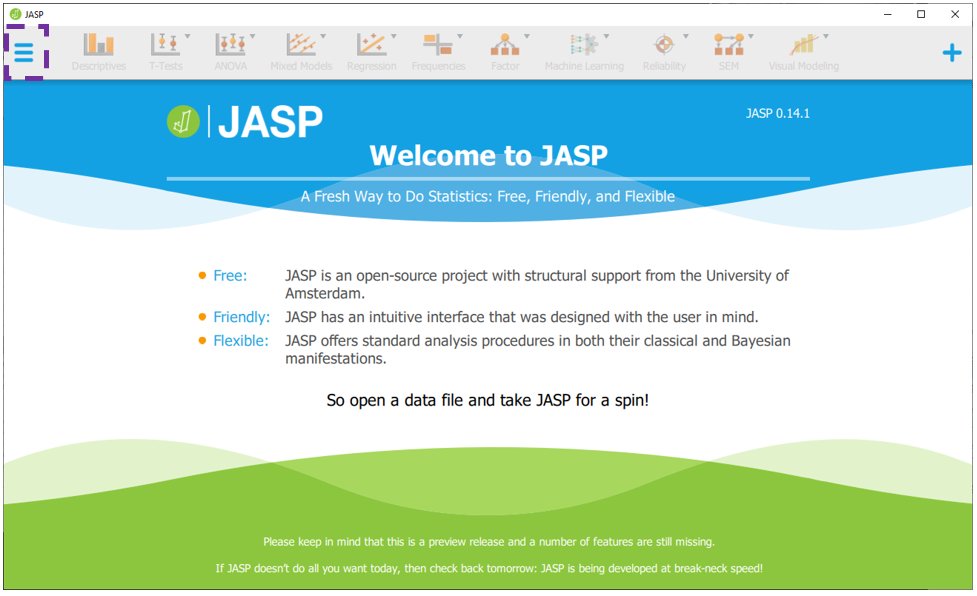
\includegraphics{./img/cap_jasp_abrir.png}

A opção \texttt{open} permite que se acesse algum diretório local específico ou se baixe os dados diretos da plataforma \emph{Open Science Framework (OSF)}. Esta versão do JASP aceita, majoritariamente, arquivos em CSV, que indica que os dados são separados por vírgulas.

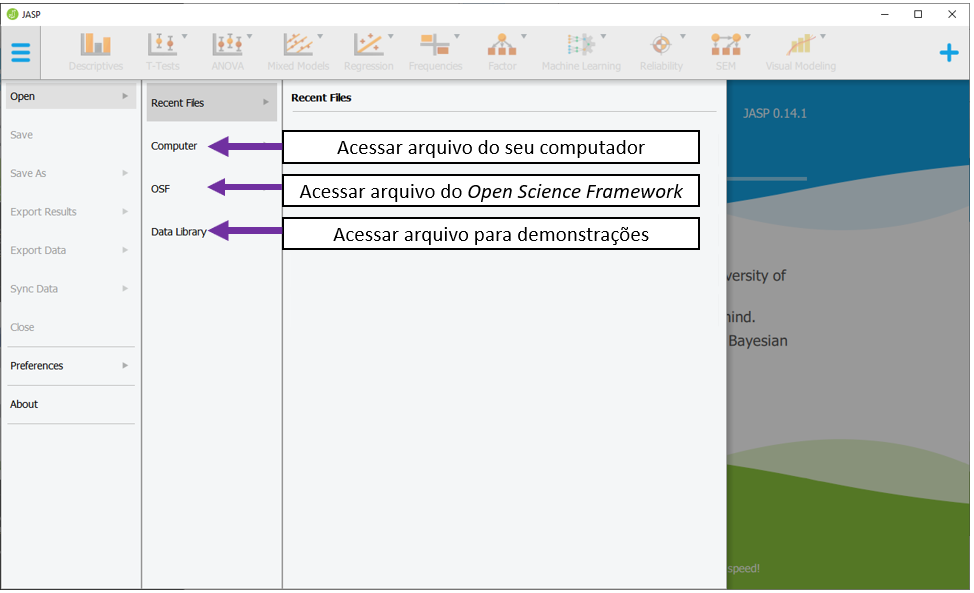
\includegraphics{./img/cap_jasp_abrir2.png}

Ao abrir algum arquivo de dados, o JASP irá apresentar os dados no centro do programa e as opções de análise na parte superior. Tenha atenção que essas telas podem variar de versão para versão.

Em relação aos dados, quase sempre o formato utilizado é o largo. Neste formato, cada coluna representa uma variável, cada linha representa um caso e cada célula (ou vetor) apresenta um valor específico.

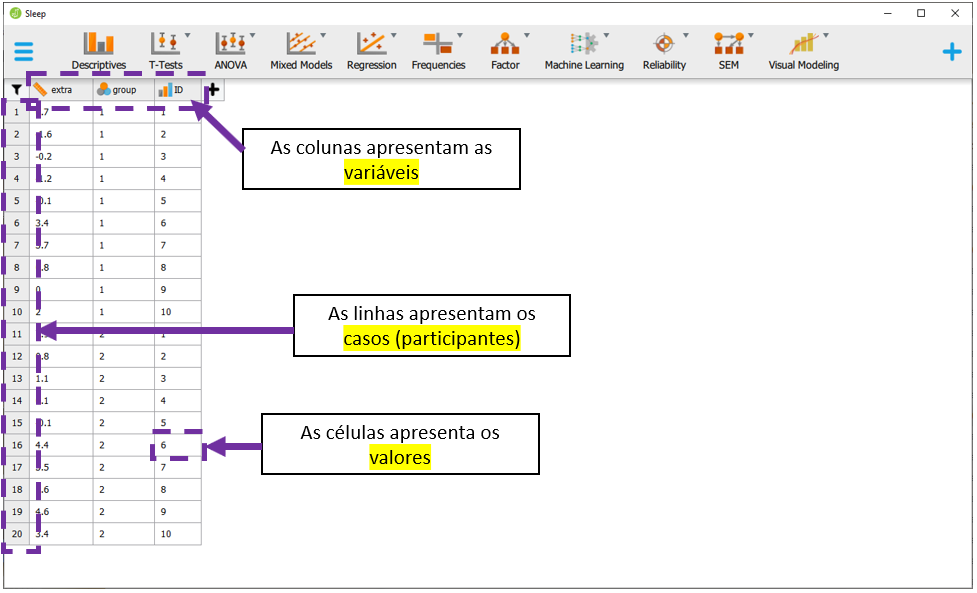
\includegraphics{./img/cap_jasp_dados.png}
O JASP adota uma simbologia específica para definir a escala (ou nível) de medida das variáveis. Isso pode ser visto no símbolo ao lado dos nomes das variáveis. Para alterar o nível, basta clicar sobre o símbolo.

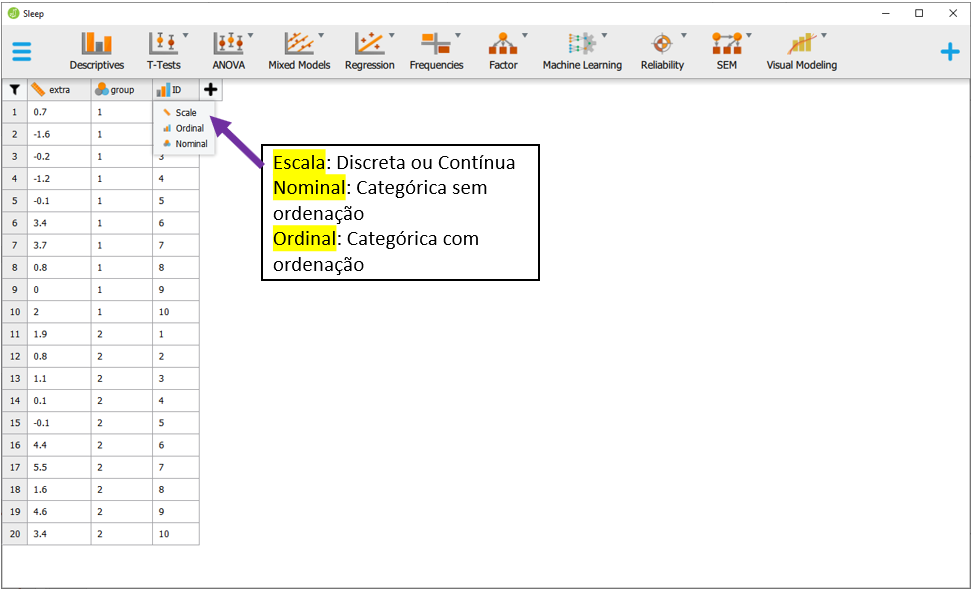
\includegraphics{./img/cap_jasp_tipo_de_dados.png}

É possível também alterar valores e rótulos das variáveis. Para isso, basta clicar no centro da variável. Uma seção na parte de cima do programa será exibida. Para fechar, é necessário clicar no X ao lado direito.

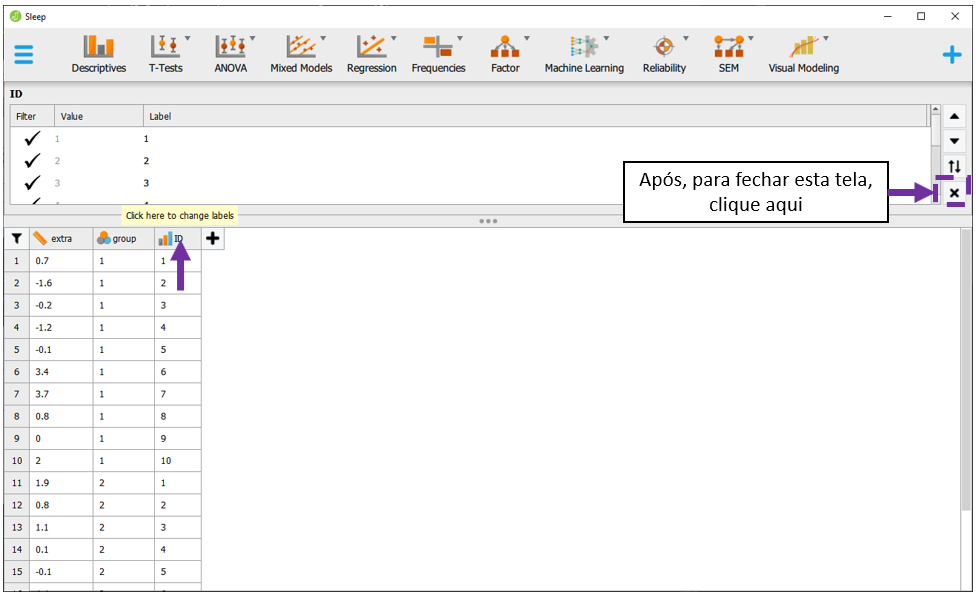
\includegraphics{./img/cap_jasp_alterar_valores.png}

Na parte superior, o JASP oferece as análises possíveis. As opções podem variar de versão para versão, mas as principais tendem a ser as seguintes.

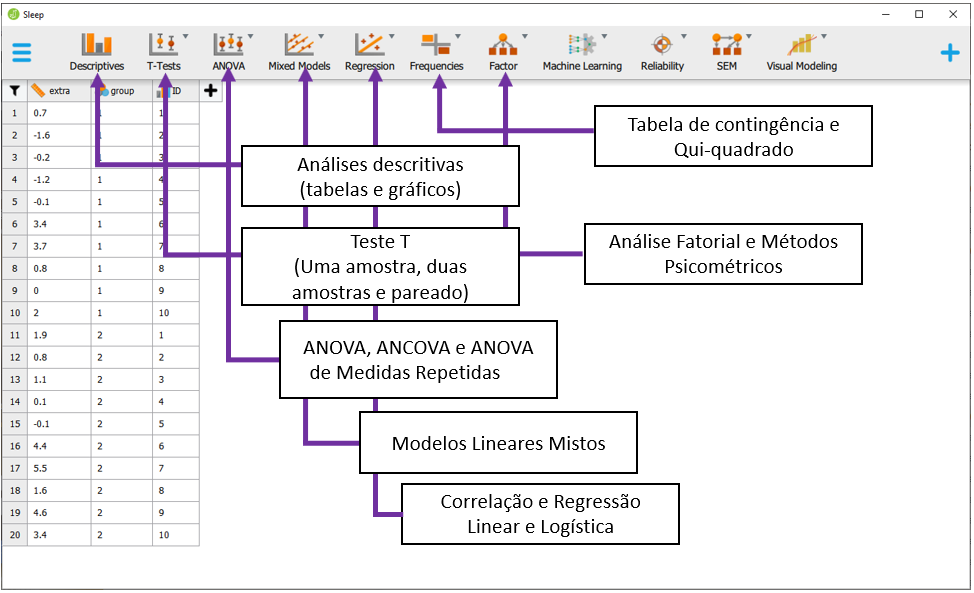
\includegraphics{./img/cap_jasp_features.png}

É possível adicionar módulos e complementos no JASP. Essas adições funcionam de maneira análoga aos pacotes do R. Para fazer isso, basta clicar na cruz azul ao lado direito.

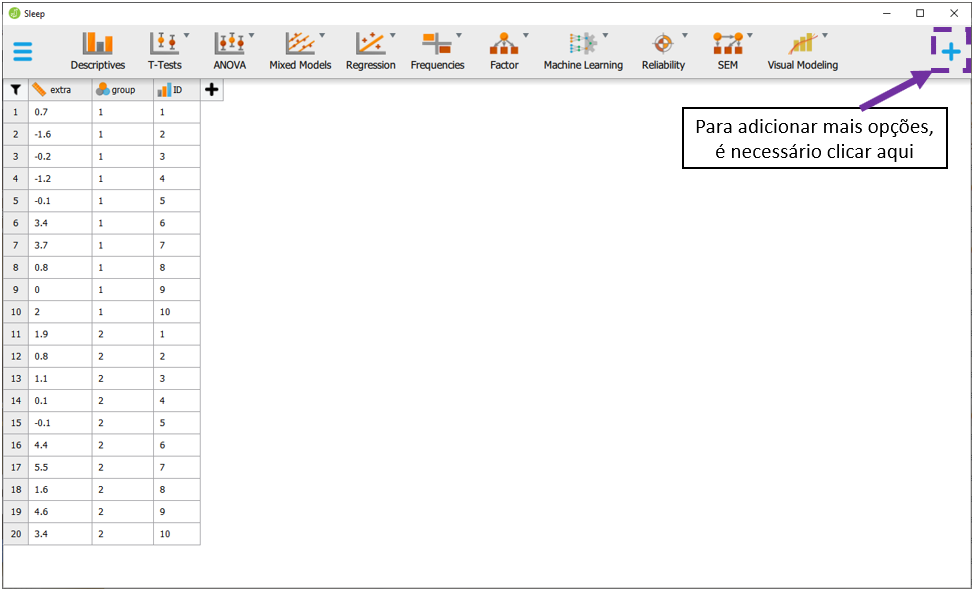
\includegraphics{./img/cap_jasp_adicionar_modulos.png}

Uma barra ao lado direito irá ser exibida. Qualquer opção pode ser selecionada e, ao fazer isso, novos botões irão aparecer na parte superior do programa.

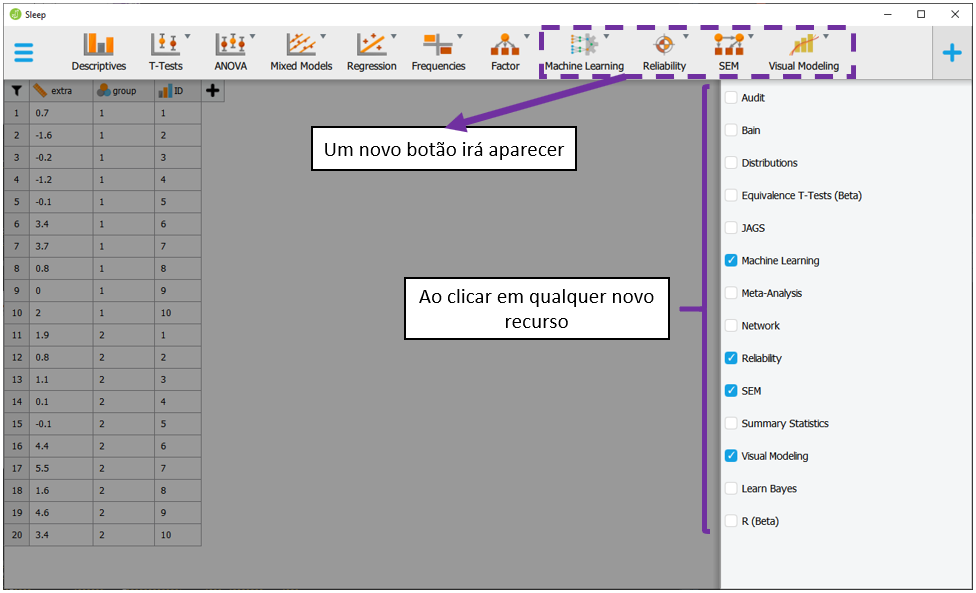
\includegraphics{./img/cap_jasp_adicionar_modulos2.png}

Finalmente, para salvar o trabalho realizado em uma sessão, deve-se clicar na símbolo de três linhas azuis e, em seguida, clicar em \texttt{Save\ as} e selecionar a pasta.. Por padrão, o formato do arquivo sera *.jasp.

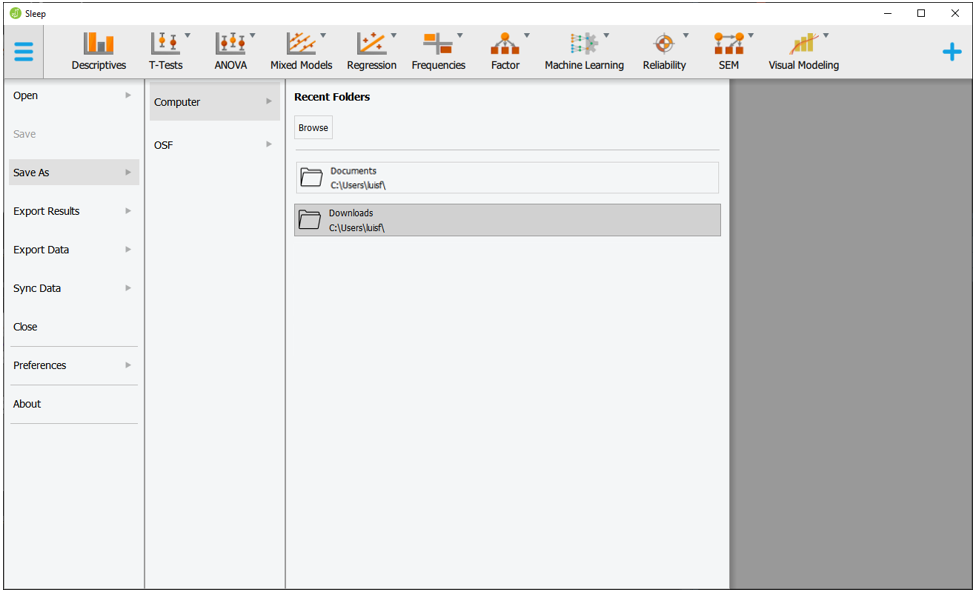
\includegraphics{./img/cap_jasp_salvar.png}

\hypertarget{resumo}{%
\section{Resumo}\label{resumo}}

\begin{explore}

\begin{enumerate}
\def\labelenumi{\arabic{enumi}.}
\tightlist
\item
  Há muitos programas e pacotes de estatística. Neste livro, o R e o JASP serão utilizados.\\
\item
  O R oferece é gratuito e um ambiente de programação e o tidyverse servirá como principal interface.\\
\item
  O JASP tem recebido grande atenção especialmente em Psicologia e as análises também serão feitas nele.\\
\end{enumerate}

\end{explore}

  \bibliography{book.bib,packages.bib}

\end{document}
